% Generado por model/metricas.py - requiere \usepackage{pgfplots}
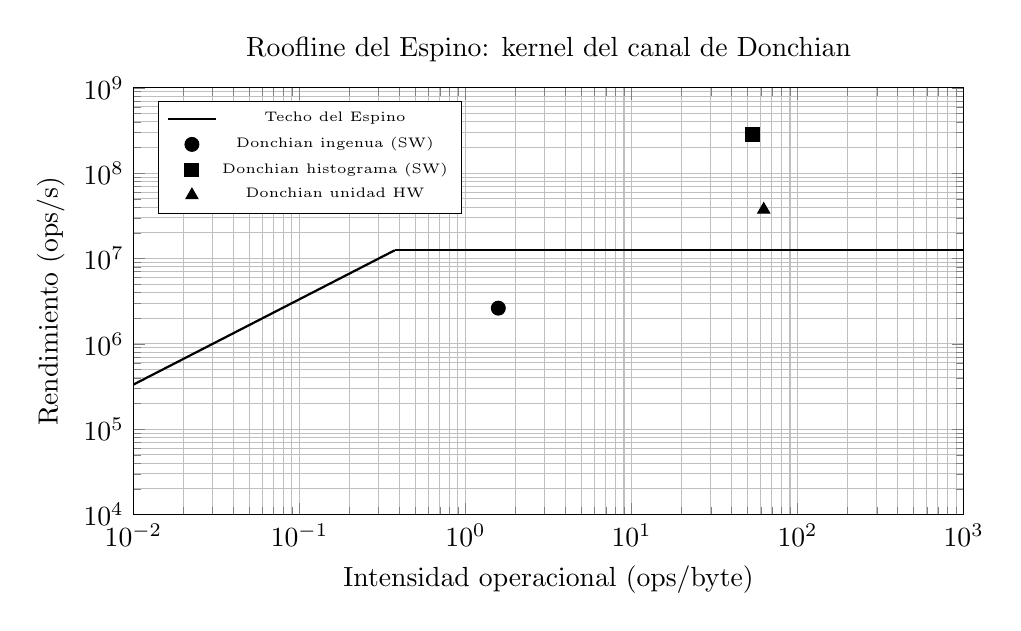
\begin{tikzpicture}
\begin{axis}[
  xmode=log, ymode=log,
  xlabel={Intensidad operacional (ops/byte)}, ylabel={Rendimiento (ops/s)},
  title={Roofline del Espino: kernel del canal de Donchian}, legend pos=north west, legend style={font=\tiny},
  xmin=0.01, xmax=1000, ymin=1e4, ymax=1e9, grid=both,
  width=\linewidth, height=7cm]
\addplot[thick, black, domain=0.01:0.375, samples=2] {3.33333e+07*x};
\addplot[thick, black, domain=0.375:1000, samples=2, forget plot] {1.25e+07};
\addlegendentry{Techo del Espino}
\addplot[only marks, mark=*, mark size=2.5pt] coordinates {(1.57563,2.6217e+06)};
\addlegendentry{Donchian ingenua (SW)}
\addplot[only marks, mark=square*, mark size=2.5pt] coordinates {(53.3915,2.82418e+08)};
\addlegendentry{Donchian histograma (SW)}
\addplot[only marks, mark=triangle*, mark size=2.5pt] coordinates {(62.5,3.73506e+07)};
\addlegendentry{Donchian unidad HW}
\end{axis}
\end{tikzpicture}
